\section{Results}

\subsection{Mono-modal registration}
Although our algorithms were designed for multi-modal image registration, it is important to first verify that the quality of the algorithms is reasonable for mono-modal registration. Table \ref{tab:monomodal_results_seg} and Figure \ref{fig:mono_graph_seg} show the average overlap score for each of 31 manually annotated anatomical regions from the IBSR database. Note that the Jaccard indices obtained with the Cross Correlation metric (i.e. ANTS) are higher than reported by \cite{Rohlfing2012}. In his experiments, he used
three resolutions with a maximum of 10, 10 and 5 iterations only. Here, we set a maximum of 100, 100 and 25 iterations, leaving the rest of the parameters unchanged. We can see that SyN with the EM metric is very competitive, but still not as good as Cross Correlation. This may be explained by the fact that CC uses a relatively large
window centered at each voxel for computing the similarity, while the EM is voxelwise. This behavior can also be observed from the results of SyN with Mutual Information (MI), which is also voxelwise and very competitve but not as good as CC. By considering neighborhoods of the same size, the performance of the Expected Cross Correlation metric is practically the same as CC. Table \ref{tab:monomodal_results_segTri_fill} shows the overlap scores over tissue types, instead of anatomical areas.

% Table generated by Excel2LaTeX from sheet 'SyNEM-Monomodal-Large'
\begin{table}[p]
\begin{adjustwidth}{-0.75cm}{}
  {\centering
    \small
    \begin{tabular}{lcccc}
    \toprule
    \textbf{}& \textbf{SyN-EM} & \textbf{SyN-ECC} & \textbf{SyN-CC} & \textbf{SyN-MI} \\
    \midrule
    \textbf{Brain-Stem} & 0.786 & \textbf{0.816} & 0.812 & 0.804 \\
    \textbf{Right-Cerebellum-Cortex} & 0.736 & \textbf{0.815} & 0.813 & 0.771 \\
    \textbf{Left-Cerebellum-Cortex} & 0.739 & \textbf{0.811} & 0.808 & 0.766 \\
    \textbf{Right-Thalamus-Proper} & 0.714 & 0.766 & \textbf{0.772} & 0.745 \\
    \textbf{Left-Thalamus-Proper} & 0.727 & 0.763 & \textbf{0.767} & 0.748 \\
    \textbf{Right-Putamen} & 0.681 & 0.748 & \textbf{0.751} & 0.712 \\
    \textbf{Left-Putamen} & 0.699 & 0.744 & \textbf{0.744} & 0.721 \\
    \textbf{Left-Cerebral-Cortex} & 0.724 & \textbf{0.739} & 0.733 & 0.687 \\
    \textbf{Right-Cerebral-Cortex} & 0.719 & \textbf{0.739} & 0.731 & 0.683 \\
    \textbf{Right-Cerebral-White-Matter} & 0.702 & \textbf{0.733} & 0.720 & 0.645 \\
    \textbf{Left-Cerebral-White-Matter} & 0.705 & \textbf{0.732} & 0.721 & 0.646 \\
    \textbf{Left-Lateral-Ventricle} & 0.731 & 0.727 & \textbf{0.732} & 0.718 \\
    \textbf{Right-Lateral-Ventricle} & 0.709 & 0.714 & \textbf{0.717} & 0.699 \\
    \textbf{Right-Cerebellum-White-Matter} & 0.576 & \textbf{0.701} & 0.691 & 0.608 \\
    \textbf{Left-Cerebellum-White-Matter} & 0.581 & \textbf{0.701} & 0.693 & 0.611 \\
    \textbf{Left-Caudate} & 0.645 & \textbf{0.671} & 0.665 & 0.666 \\
    \textbf{Right-Caudate} & 0.620 & \textbf{0.655} & 0.647 & 0.651 \\
    \textbf{Right-VentralDC} & 0.612 & 0.651 & \textbf{0.652} & 0.628 \\
    \textbf{Left-VentralDC} & 0.622 & \textbf{0.651} & 0.650 & 0.631 \\
    \textbf{Right-Pallidum} & 0.498 & \textbf{0.622} & 0.620 & 0.582 \\
    \textbf{Right-Hippocampus} & 0.572 & \textbf{0.621} & 0.620 & 0.575 \\
    \textbf{Left-Pallidum} & 0.524 & \textbf{0.615} & 0.614 & 0.583 \\
    \textbf{Left-Hippocampus} & 0.574 & \textbf{0.610} & 0.609 & 0.564 \\
    \textbf{4th-Ventricle} & 0.551 & 0.606 & \textbf{0.608} & 0.574 \\
    \textbf{3rd-Ventricle} & 0.527 & 0.544 & \textbf{0.547} & 0.515 \\
    \textbf{Left-Amygdala} & 0.444 & 0.519 & \textbf{0.519} & 0.484 \\
    \textbf{Right-Amygdala} & 0.411 & 0.513 & \textbf{0.514} & 0.458 \\
    \textbf{Left-Accumbens-area} & 0.451 & 0.500 & \textbf{0.500} & 0.462 \\
    \textbf{Right-Accumbens-area} & 0.433 & 0.490 & \textbf{0.490} & 0.443 \\
    \textbf{Right-Inf-Lat-Vent} & 0.177 & 0.230 & \textbf{0.232} & 0.162 \\
    \textbf{Left-Inf-Lat-Vent} & 0.190 & 0.228 & \textbf{0.233} & 0.167 \\
    \hline
    \textbf{Average (std.)} & 0.593 (0.148) & 0.644 (0.142) & 0.643 (0.140) & 0.603 (0.149) \\
    \textbf{Rank-1 count} & 0 & 16 & 15 & 0 \\
    \textbf{Rank-2 count} & 1 & 14 & 14 & 2 \\
    \textbf{Rank-3 count} & 9 & 1 & 2 & 19 \\
    \bottomrule
    \end{tabular}}%
    \caption{Comparison of the registration performance (measured by the Jaccard index over 31 anatomical regions) of the Greedy SyN algorithm with EM, ECC, CC and MI metrics.
The Jaccard indices were averaged over 306 monomodal registrations. Rank-$k$ counts show the number of anatomical regions for which each
method ranked $k$ among the four methods under comparison. Top performer (rank-1) for each region is highlighted. }
  \label{tab:monomodal_results_seg}%
\end{adjustwidth}
\end{table}%

% Table generated by Excel2LaTeX from sheet 'SyNEM-Monomodal-Large'
\begin{table}[htbp]
  \centering
  {\small
    \begin{tabular}{rrrr}
    \toprule
    \textbf{} & \textbf{SyN-EM} & \textbf{SyN-ECC} & \textbf{SyN-CC} \\
    \midrule
    \textbf{Background} & 0.994 & 0.995 & \textbf{0.995} \\
    \textbf{CSF} & 0.335 & 0.349 & \textbf{0.359} \\
    \textbf{Gray Matter} & 0.740 & \textbf{0.765} & 0.759 \\
    \textbf{White Matter} & 0.703 & \textbf{0.739} & 0.728 \\
    \bottomrule
    \end{tabular}%
    \caption{Comparison of the registration performance (measured by the Jaccard index over Background, CSF, GM and WM)of the Greedy SyN algorithm with EM, ECC and CC metrics. The Jaccard
indices were averaged over 306 monomodal registrations. Top performer for each region is highlighted.}
  \label{tab:monomodal_results_segTri_fill}}%
\end{table}%


\begin{figure}[t!]
\centering
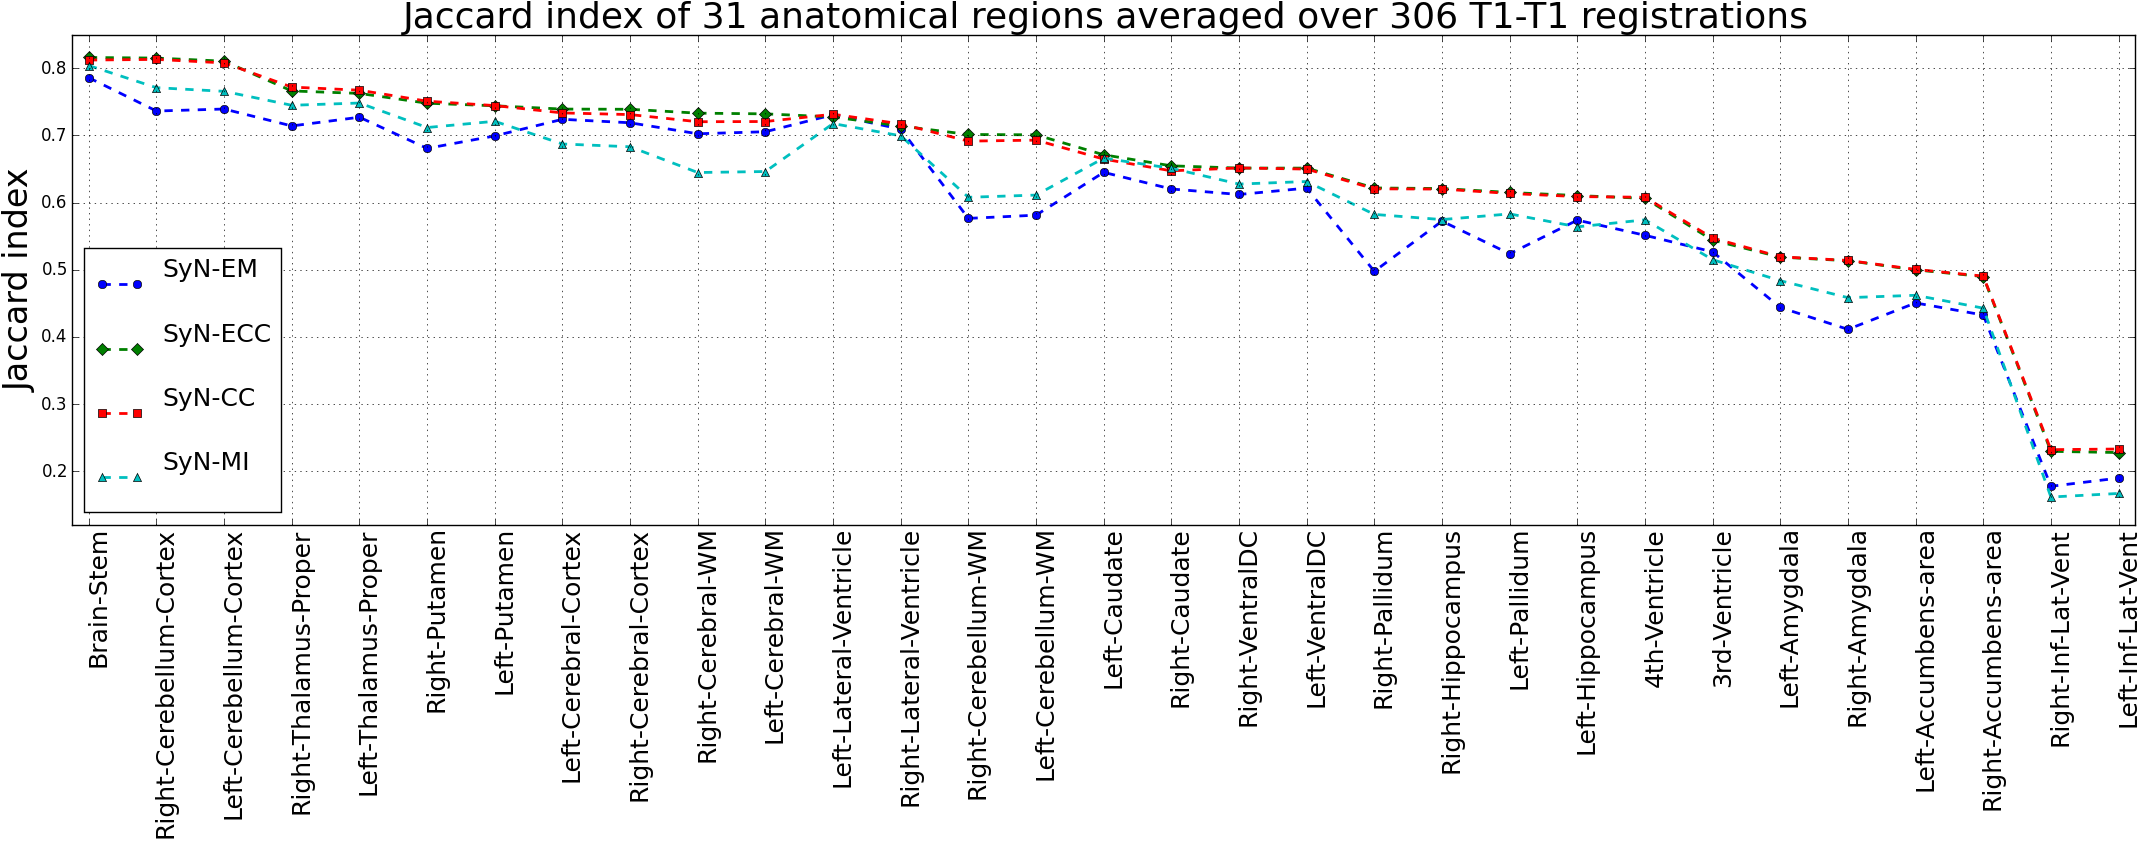
\includegraphics[width=1.0\linewidth]{./images/mono_lines_seg.png}\\
\caption{Comparison of the registration performance (measured by the Jaccard index over 31 anatomical regions) of the Greedy SyN algorithm with EM, ECC, CC and MI metrics. The Jaccard
indices were averaged over 306 monomodal registrations.}
\label{fig:mono_graph_seg}
\end{figure}

\subsection{Multi-modal registration}\label{sec:multimodal_results}
The cross-correlation metric is occasionally used for some multi-modal image registration tasks. The reason is that the metric's optimality is reached when the relationship between the two image modalities is locally affine. However, in general, this condition is not met. To illustrate this, we used the Brainweb synthetic template \citep{Cocosco1997, Kwan1999}. Brainweb provides two perfectly aligned, realistically simulated brain MR images in T1 and T2 modalities. Ideally, a multi-modal registration method should return the identity transformation to register these perfectly aligned images. Figure \ref{fig:t1_t2_reg_pannel} depicts the result of registering the images using the SyN algorithm with four different metrics. We can see that using the CC metric, the cortex was (incorrectly) strongly deformed: the deformation field maximizing the cross correlation between the two multi-modal images does not coincides with the deformation field correctly aligning the images. This effect is less pronounced using the EM metric. Despite the deformation field is not exactly zero using the ECC metric, the deformations are much smaller. Using MI, the moving image is left almost unchanged with a maximum displacement of 0.4mm and an average of 0.06mm (Table \ref{tab:deformation_magnitude}). The reason that the CC metric does not perform well in this experiment is that the relationship between the two modalities is not locally affine (Fig. \ref{fig:transfers}). Despite the MI metric successfully reaches its maximum very close to the identity transformation, we must consider that it depends on an accurate computation of the joint and marginal intensity distributions of both modalities, which is not known {it a priori} and needs to be iteratively refined as the registration evolves. By providing two perfectly aligned images as input, the intensity distributions can be accurately computed from iteration one, which is an unrealistic scenario. Thus, a more realistic validation protocol is required to quantitatively evaluate the metrics under comparison in the multi-modal case.

\begin{table}[htbp]
  \centering
  {\small
    \begin{tabular}{ccccc}
    \toprule
    \textbf{} & \textbf{SyN-CC} & \textbf{SyN-EM} & \textbf{SyN-ECC} &\textbf{SyN-MI} \\
    \midrule
    \textbf{Mean}    & 2.98  & 0.21 & 0.15 & 0.06 \\
    \textbf{Maximum} & 11.70 & 3.90 & 2.60 & 0.40\\
    \bottomrule
    \end{tabular}%
    \caption{Magnitude (in millimeters) of the deformation field obtained by registering two perfectly aligned multi-modal images using SyN with four different metrics (ideally, the deformation field should be zero). First row shows the average norm of all displacement
    vectors, while second row shows the maximum norm.}
  \label{tab:deformation_magnitude}}%
\end{table}%


\begin{figure}[t!]
\centering
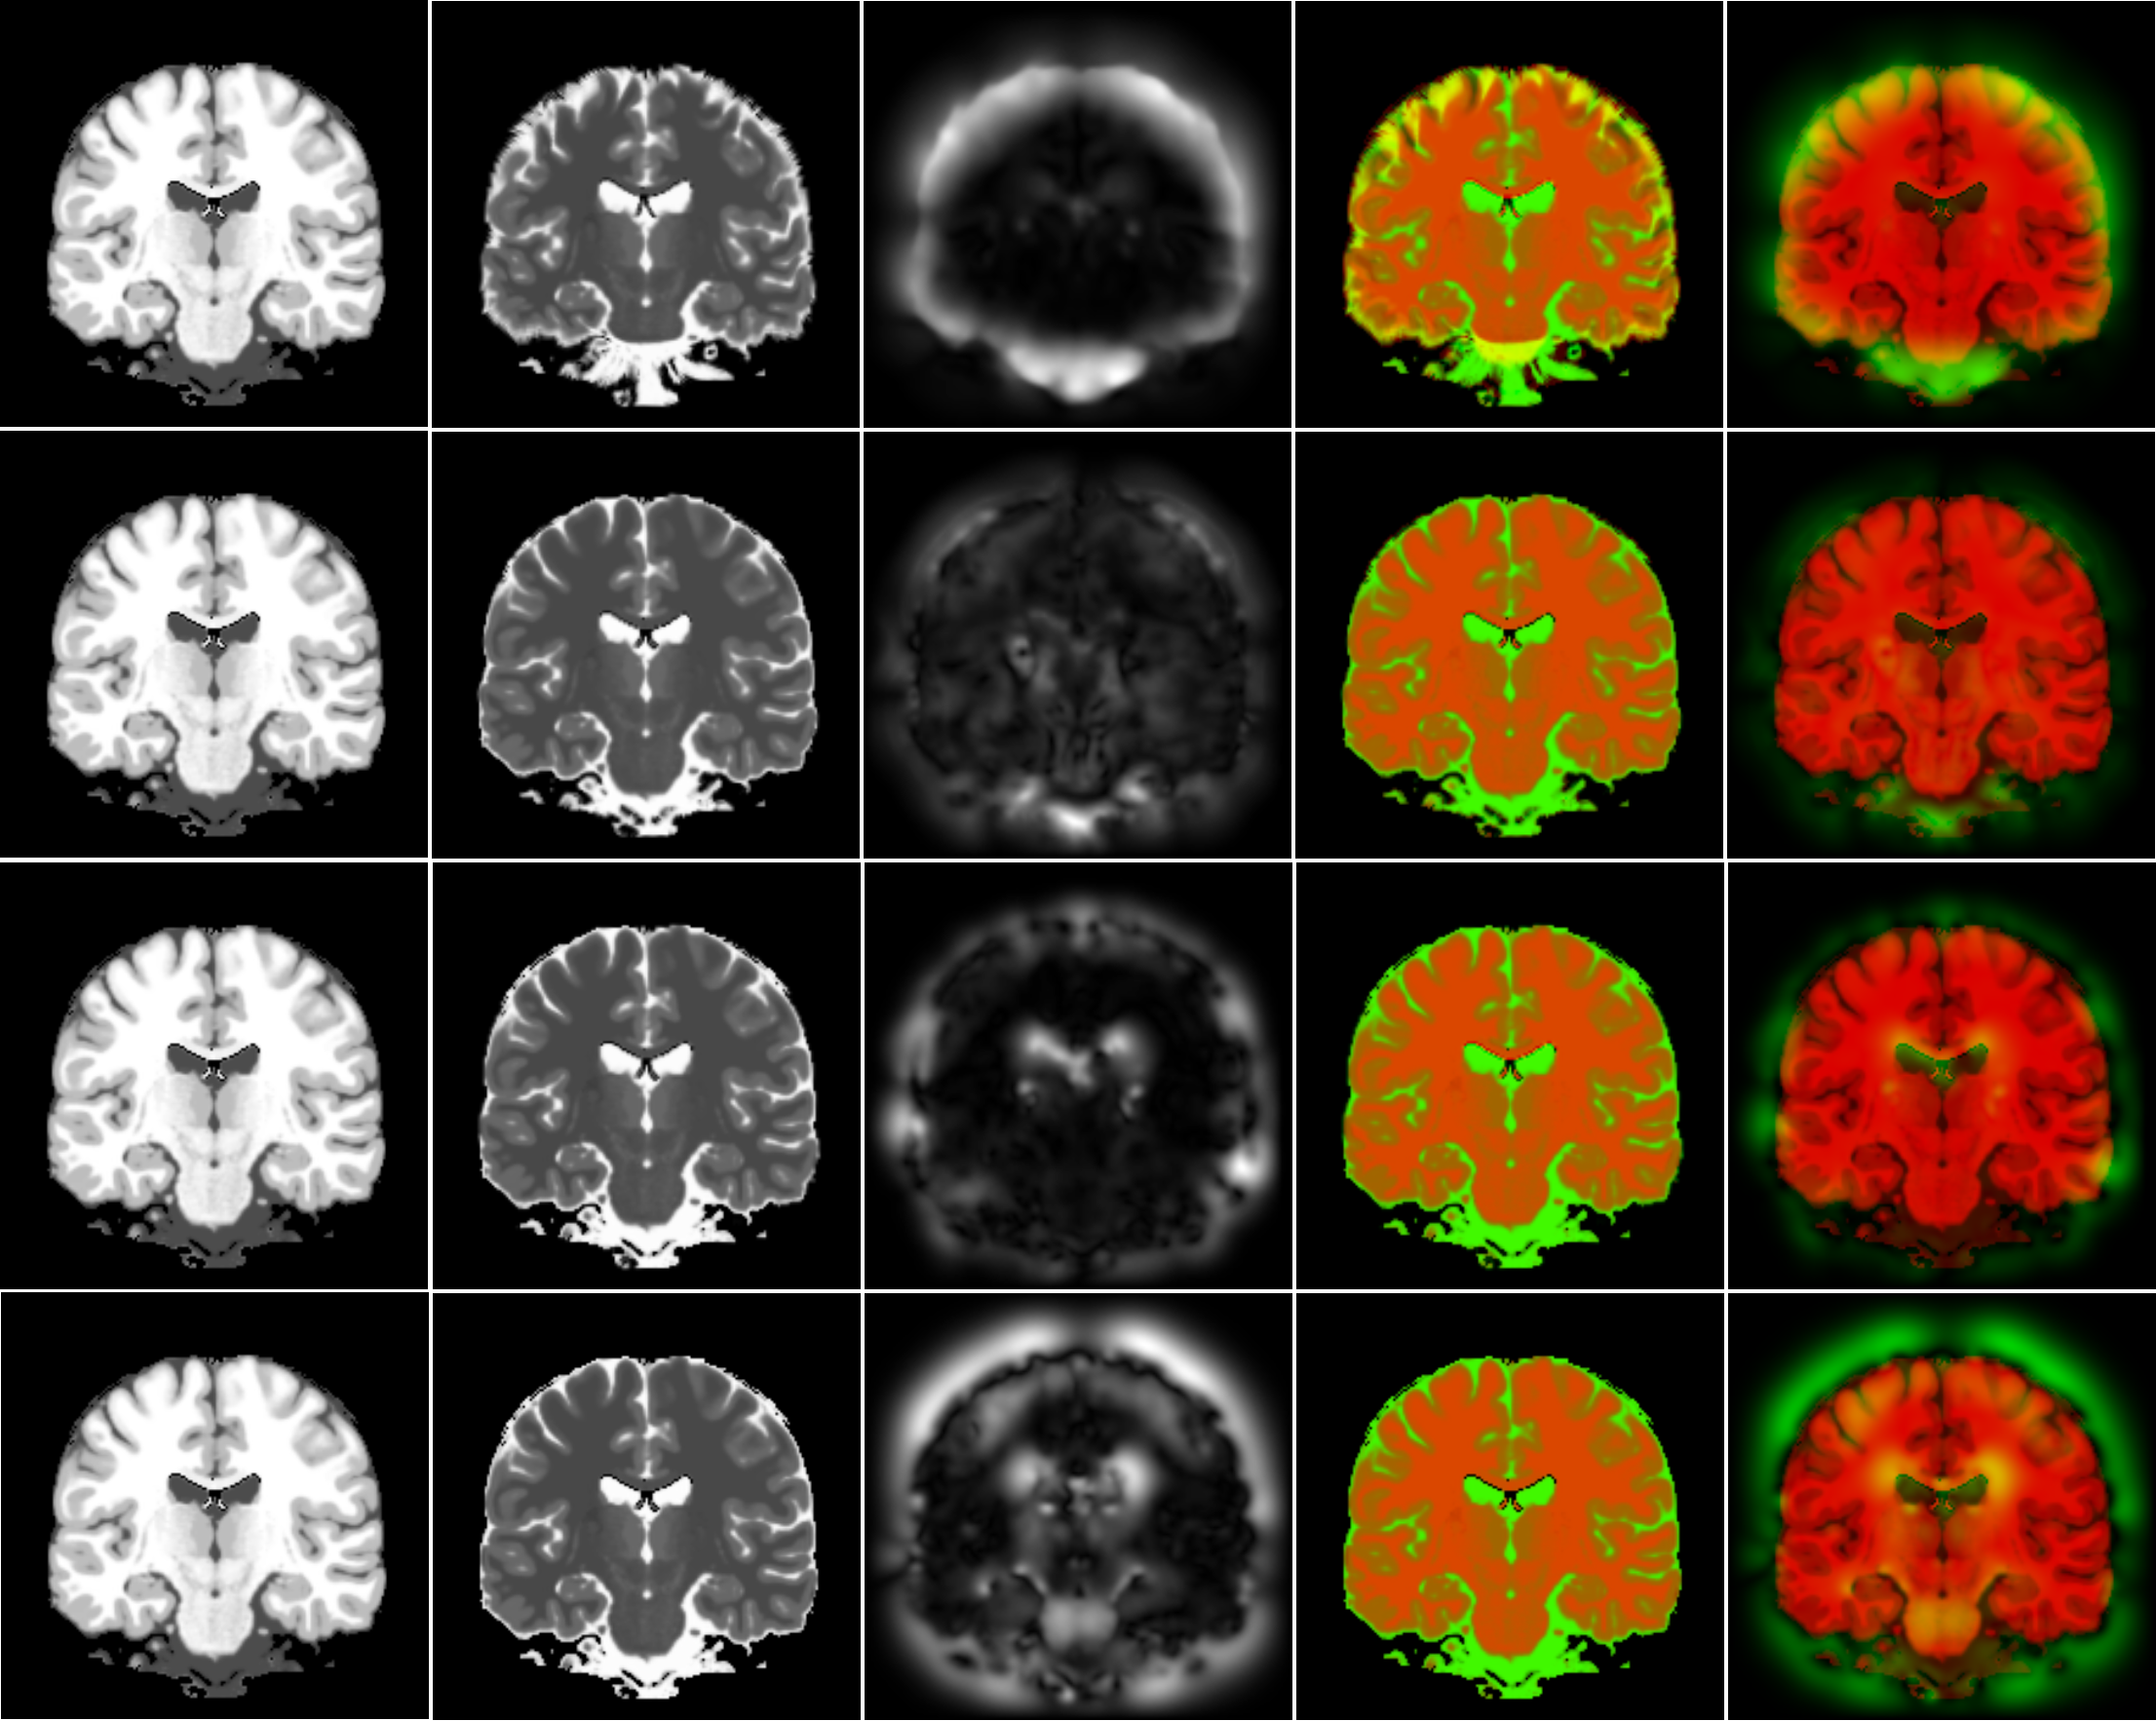
\includegraphics[width=1.0\linewidth]{./images/t1_t2_reg_pannel.png}
\caption{T2 brain image registered towards T1 using the greedy SyN algorithm with different metrics. Since both images are perfectly aligned, the expected result is a zero deformation field. Row 1: using the CC metric, the cortex is clearly distorted. Row 2: with the EM metric deformations are less visible. Row 3: with the ECC metric deformations are smaller than with the EM metric. Row 4: the MI metric leaves the image almost unchanged (see Table \ref{tab:deformation_magnitude} for detailed numerical results). Note that, with exception of the CC metric, the largest deformations occur outside of the region of interest, which is a result of the regularization term.}
\label{fig:t1_t2_reg_pannel}
\end{figure}

Unfortunately, to the best of our knowledge, there are no manually annotated multi-modality data publicly available to evaluate the registration performance quantitatively. Instead, we generated synthetic T2 images for all IBSR T1 images by following the procedure illustrated in Fig. (\ref{fig:semi_synthetic_image_creation}). We first register the Brainweb T1 template (which plays the role of moving image) towards each IBSR T1 image (which play the role of fixed image) using ANTs with the CC metric (a mono-modal registration problem), which has consistently ranked first in the most extensive evaluations of mono-modal registration algorithms \citep{Klein2009, Klein2010, Rohlfing2012}. Then we applied the obtained deformation field to the Brainweb T2 template. The transfer function from the real T1 image to the warped T2 template is computed as the average T2 intensity associated to each T1 intensity. The computed transfer function is then applied to the real IBSR T1 image obtaining a ``perfectly aligned'' realistic synthetic T2 image for each IBSR volume, therefore the annotations remain exactly the same as the T1 counterparts and we are able to compute the overlap scores as before. Note that the number of registrations we need to perform is now 612 because we can use the T2 modality either as the moving or the fixed image. Table \ref{tab:multimodal_results_seg} and Figure \ref{fig:multi_seg} show results similar to Table \ref{tab:monomodal_results_seg} and Figure \ref{fig:mono_graph_seg} but this time averaged over 612 multimodal registrations. Note how the performance of the CC metric strongly drops while EM and ECC are less affected by the change of modality. Table \ref{tab:multimodal_results_segTri_fill} shows the overlap scores of tissue types, where the same behavior can be observed.\\

\pagebreak
\begin{figure}[t!]
\centering
    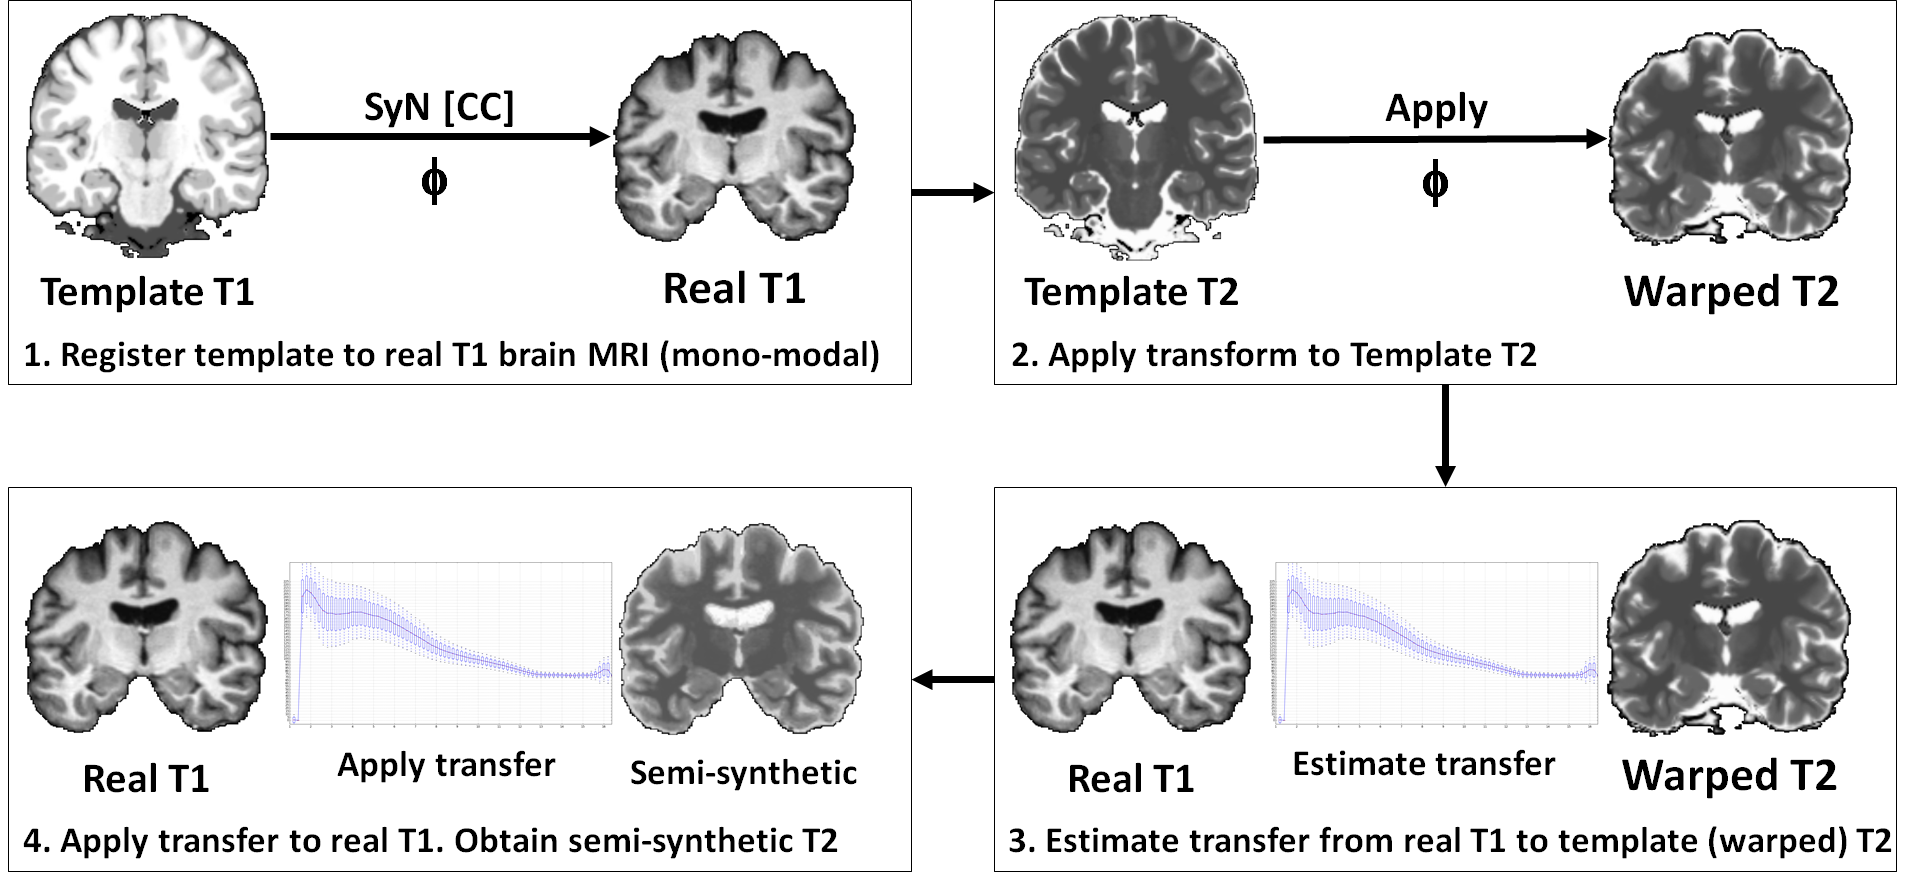
\includegraphics[width=\linewidth]{./images/semi_synthetic_image_creation.png}
    \caption{Semi-synthetic, manually annotated images for quantitative evaluation of multi-modal non-linear image registration algorithms.}
\label{fig:semi_synthetic_image_creation}
\end{figure}

The Brainweb template also provides us with a simulation of a proton density (PD) image for the same brain anatomy. This allows us to repeat the procedure described above for each pair of three modalities, T1, T2 and PD, which results in 3 mono-modal and 3 multi-modal registration experiments. For the sake of brevity, Figure \ref{fig:all_pairs_boxplots} depicts a summary of the results obtained over all pairs of modalities. For each pair of registered images, we compute the average Jaccard index of all anatomical regions. Each boxplot in Figure \ref{fig:all_pairs_boxplots} corresponds to the set of all 306 (mono-modal) or 612 (multi-modal) average scores for that particular method and that particular pair of modalities. We can observe that the CC metric performs very well for all mono-modal experiments (diagonal graphs), but it is severely affected in the multi-modal case (off-diagonal graphs). The ECC metric performs practically the same as CC in the mono-modal case, but is less affected in the multi-modal case. By measuring the similarity of local windows instead of individual voxels, the ECC metric outperforms the EM and MI metrics in all cases.

\begin{figure}[t!]
\centering
    \subfloat[]{\label{fig:T1T2}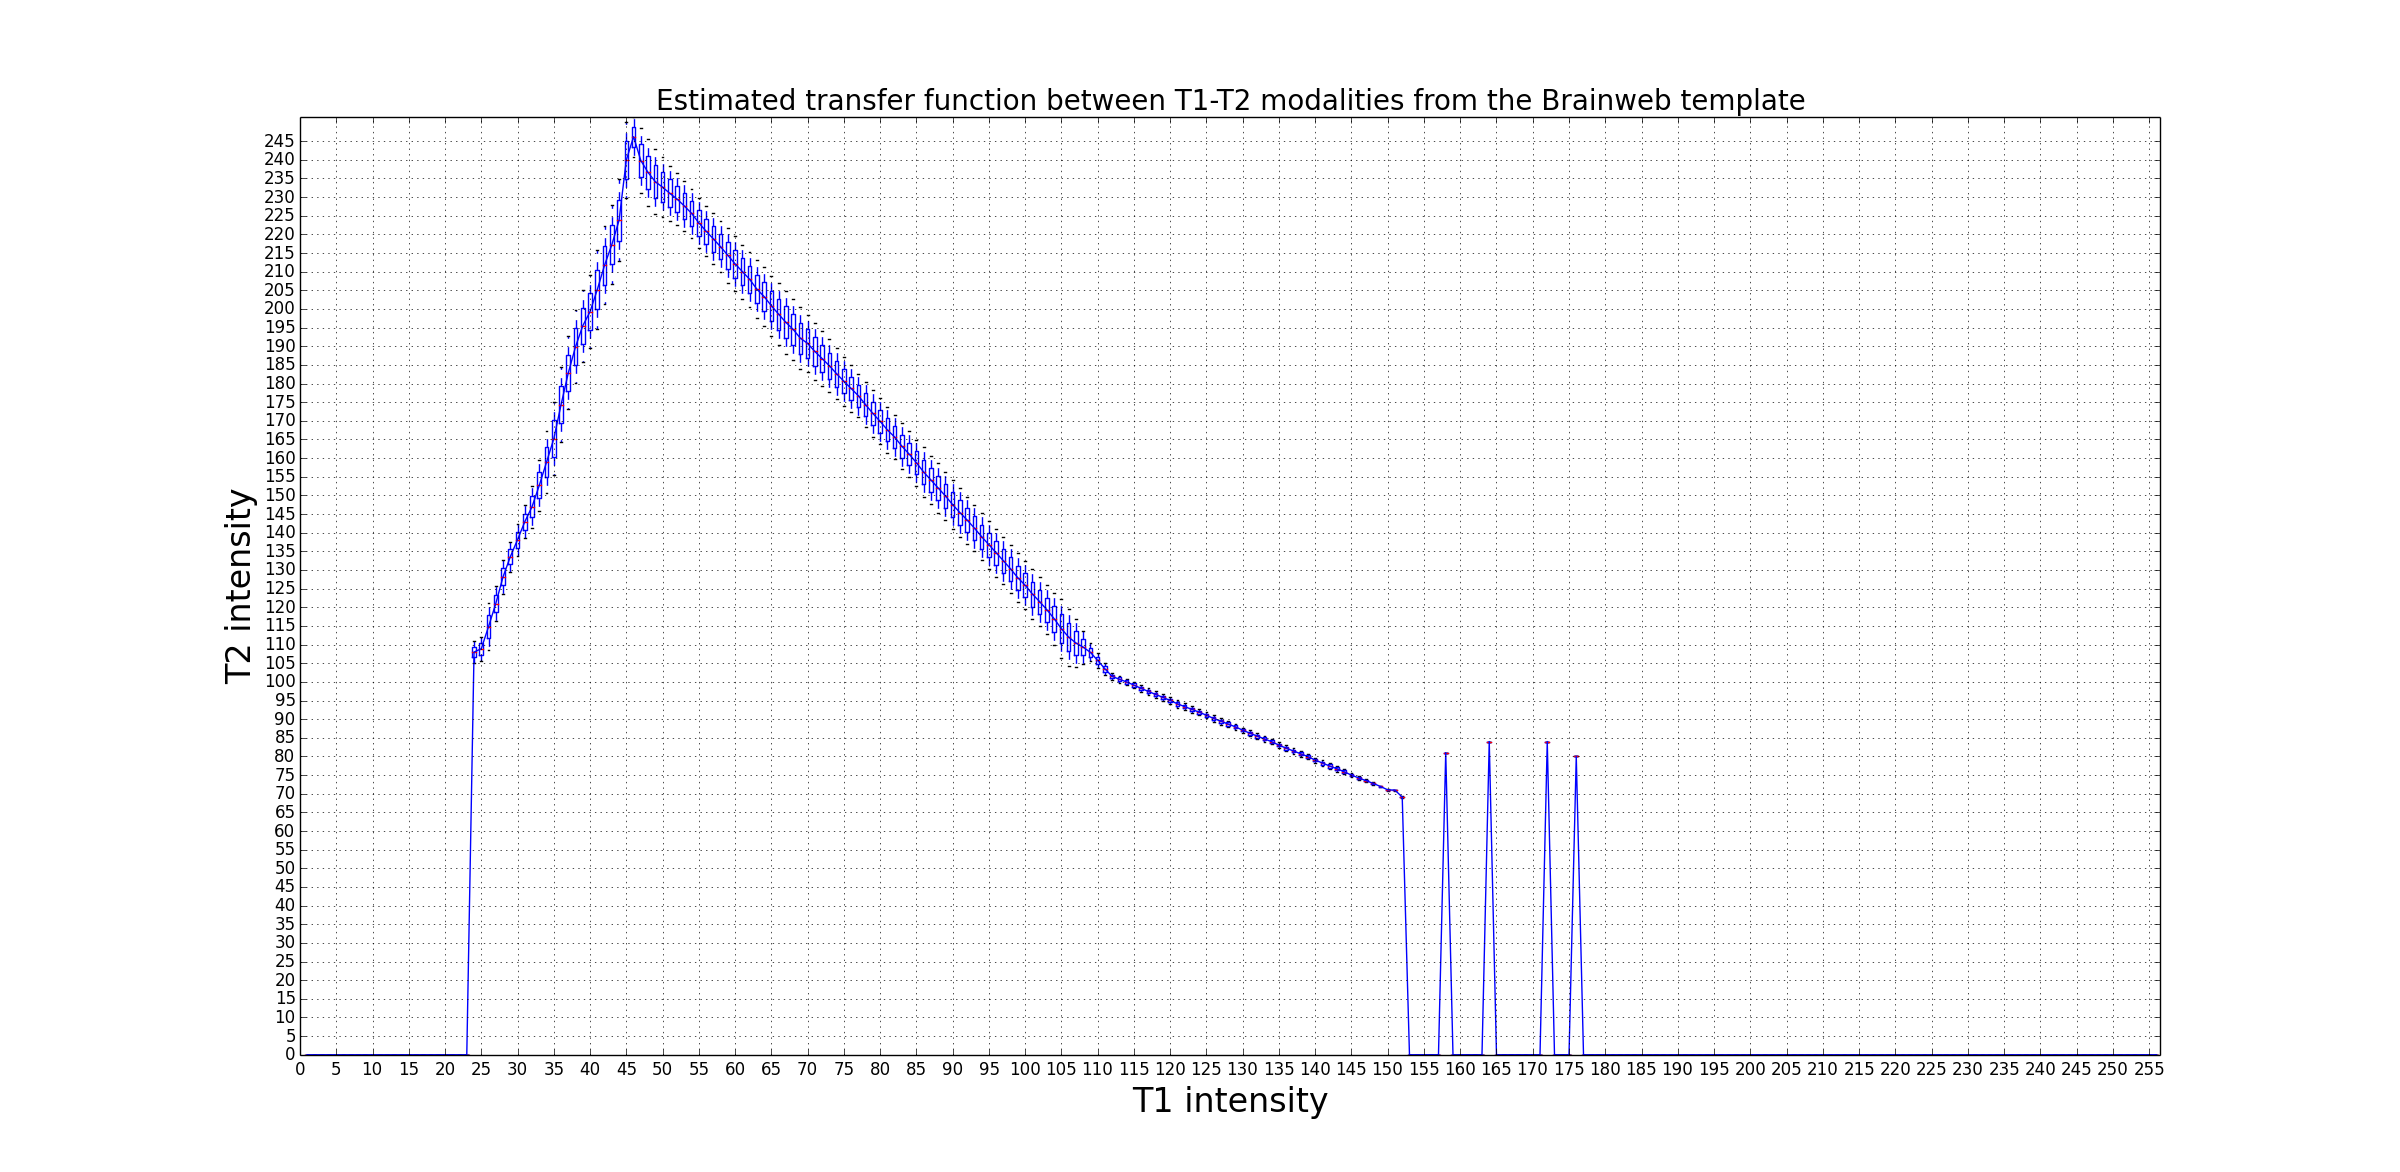
\includegraphics[width=0.5\linewidth]{./images/t1_t2_transfer_brainweb.png}}
    \subfloat[]{\label{fig:T2T1}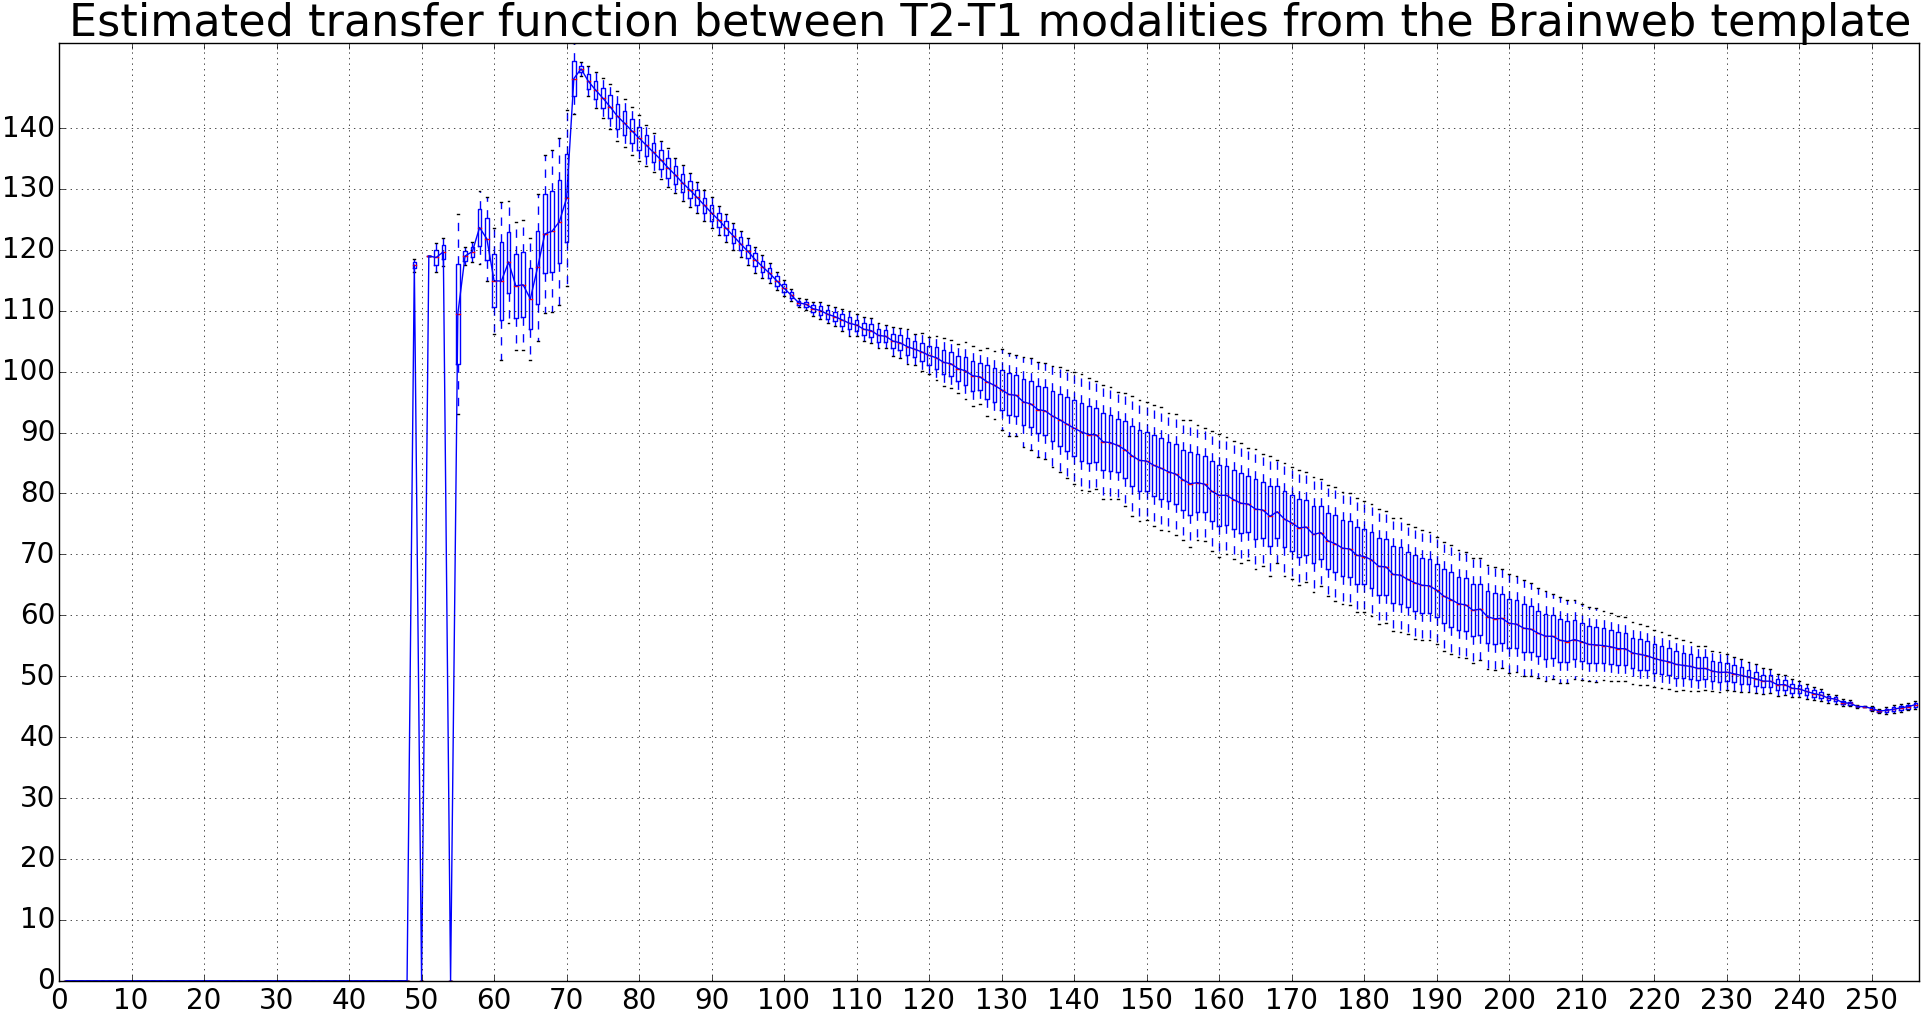
\includegraphics[width=0.5\linewidth]{./images/t2_t1_transfer_brainweb.png}}\\
    \caption{Estimated transfer functions, according to eq. \eqref{eq:expectation_transfer} using the Brainweb template where the T1 template is $I$ and the T2 template is $J$
    (since the two templates are perfectly aligned, the transformations $\phi_{I}, \phi_{J}$ are identities). (a) Estimated $\overline{Y}(x), 0\leq x \leq 255$, (b) Estimated $\overline{Z}(x), 0\leq x \leq 255$. The height of each box is proportional to $\sigma_{Y}$ and $\sigma_{Z}$, respectively. The fact that the variances are not zero indicates that there is no exact transfer function between the two modalities. Larger variances indicate larger uncertainty in the estimated transfer function, which is used by the EM metric to weigh the observed intensities. These transfers correspond to the T1-T2 template images and are used for illustrative purposes only. To generate the semi-synthetic images used for quantitative validation, a different transfer must be computed from each IBSR T1 image to the template T2 image (see Fig. \ref{fig:semi_synthetic_image_creation}).}
\label{fig:transfers}
\end{figure}


%\begin{figure}[H]
%\centering
%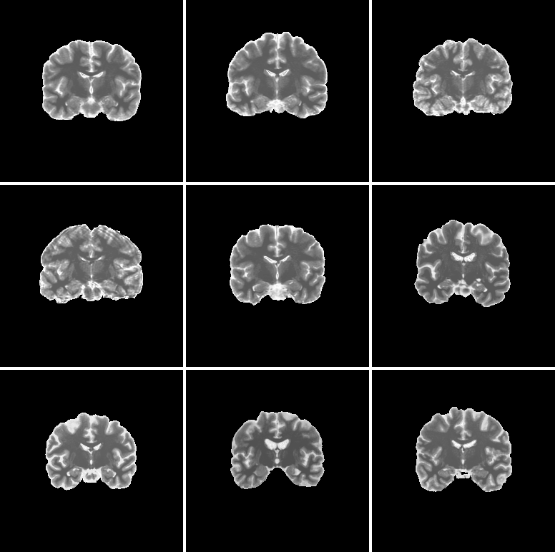
\includegraphics[width=1.0\linewidth]{./images/semi_synthetic.png}\\
%\caption{First 9 T2 images generated from the real IBSR T1 images and the T2 Brainweb template (see text). Since the anatomy remained unchanged, the manual annotations are exactly %the same as the corresponding T1 images. Notice that, since several T1 intensities map to the same T2 intensity, the transfer from T2 to T1 is not monomodal (see Fig. %\ref{fig:transfers} for an example of the transfers' shape).}
%\label{fig:semi_synthetic}
%\end{figure}

% Table generated by Excel2LaTeX from sheet 'SyNEM-Multi-Large'
\begin{table}[htbp]
  \centering
  {\small
    \begin{tabular}{rrrr}
    \toprule
          & \textbf{SyN-ECC} & \textbf{SyN-EM} & \textbf{SyN-CC} \\
    \midrule
    \textbf{Right-Thalamus-Proper:} & \textbf{0.758} & 0.716 & 0.756 \\
    \textbf{Left-Thalamus-Proper:} & \textbf{0.754} & 0.727 & 0.752 \\
    \textbf{Left-Lateral-Ventricle:} & 0.709 & 0.706 & \textbf{0.733} \\
    \textbf{Right-Lateral-Ventricle:} & 0.696 & 0.687 & \textbf{0.718} \\
    \textbf{Left-Putamen:} & \textbf{0.740} & 0.699 & 0.683 \\
    \textbf{Right-Putamen:} & \textbf{0.742} & 0.684 & 0.676 \\
    \textbf{Brain-Stem:} & \textbf{0.790} & 0.786 & 0.663 \\
    \textbf{Left-Cerebellum-Cortex:} & \textbf{0.765} & 0.729 & 0.649 \\
    \textbf{Right-Cerebellum-Cortex:} & \textbf{0.769} & 0.729 & 0.645 \\
    \textbf{Left-Caudate:} & \textbf{0.652} & 0.628 & 0.637 \\
    \textbf{Right-Caudate:} & \textbf{0.636} & 0.606 & 0.618 \\
    \textbf{Right-Cerebral-White-Matter:} & \textbf{0.723} & 0.683 & 0.571 \\
    \textbf{Left-Cerebral-White-Matter:} & \textbf{0.722} & 0.685 & 0.570 \\
    \textbf{Left-Cerebral-Cortex:} & \textbf{0.700} & 0.699 & 0.558 \\
    \textbf{Right-Cerebral-Cortex:} & \textbf{0.697} & 0.694 & 0.548 \\
    \textbf{4th-Ventricle:} & \textbf{0.583} & 0.546 & 0.543 \\
    \textbf{Right-Hippocampus:} & \textbf{0.610} & 0.570 & 0.503 \\
    \textbf{Right-VentralDC:} & \textbf{0.642} & 0.616 & 0.499 \\
    \textbf{Right-Pallidum:} & \textbf{0.606} & 0.528 & 0.499 \\
    \textbf{Left-Pallidum:} & \textbf{0.602} & 0.545 & 0.495 \\
    \textbf{3rd-Ventricle:} & \textbf{0.517} & 0.511 & 0.492 \\
    \textbf{Left-VentralDC:} & \textbf{0.640} & 0.622 & 0.491 \\
    \textbf{Left-Hippocampus:} & \textbf{0.600} & 0.567 & 0.488 \\
    \textbf{Left-Cerebellum-White-Matter:} & \textbf{0.688} & 0.582 & 0.485 \\
    \textbf{Right-Cerebellum-White-Matter:} & \textbf{0.690} & 0.579 & 0.476 \\
    \textbf{Left-Amygdala:} & \textbf{0.505} & 0.447 & 0.360 \\
    \textbf{Right-Amygdala:} & \textbf{0.497} & 0.415 & 0.339 \\
    \textbf{Right-Accumbens-area:} & \textbf{0.483} & 0.433 & 0.339 \\
    \textbf{Left-Accumbens-area:} & \textbf{0.494} & 0.448 & 0.338 \\
    \textbf{Left-Inf-Lat-Vent:} & \textbf{0.219} & 0.178 & 0.194 \\
    \textbf{Right-Inf-Lat-Vent:} & \textbf{0.219} & 0.164 & 0.178 \\
    \bottomrule
    \end{tabular}}%
    \caption{Comparison of the registration performance (measured by the Jaccard index over 31 anatomical regions) of the Greedy SyN algorithm with EM, ECC and CC metrics. The Jaccard
indices were averaged over 612 multimodal registrations. Top performer for each region is highlighted.}
  \label{tab:multimodal_results_seg}%
\end{table}%

% Table generated by Excel2LaTeX from sheet 'SyNEM-Multi-Large'
\begin{table}[htbp]
  \centering
  {\small
    \begin{tabular}{ccccc}
    \toprule
          & \textbf{SyN-EM} & \textbf{SyN-ECC} & \textbf{SyN-CC} & \textbf{SyN-MI} \\
    \midrule
    \textbf{Background} & 0.993 & 0.995 & 0.990 & \textbf{0.995} \\
    \textbf{CSF} & 0.275 & \textbf{0.335} & 0.157 & 0.325 \\
    \textbf{Gray Matter} & 0.718 & \textbf{0.742} & 0.597 & 0.691 \\
    \textbf{White Matter} & 0.685 & \textbf{0.718} & 0.572 & 0.622 \\
    \bottomrule
    \end{tabular}}%
  \caption{Comparison of the registration performance (measured by the Jaccard index over Background, CSF, GM and WM)of the Greedy SyN algorithm with EM, ECC, CC and MI metrics.
The Jaccard indices were averaged over 612 multimodal registrations. Top performer for each region is highlighted.}
  \label{tab:multimodal_results_segTri_fill}%
\end{table}%


\begin{figure}[t!]
\centering
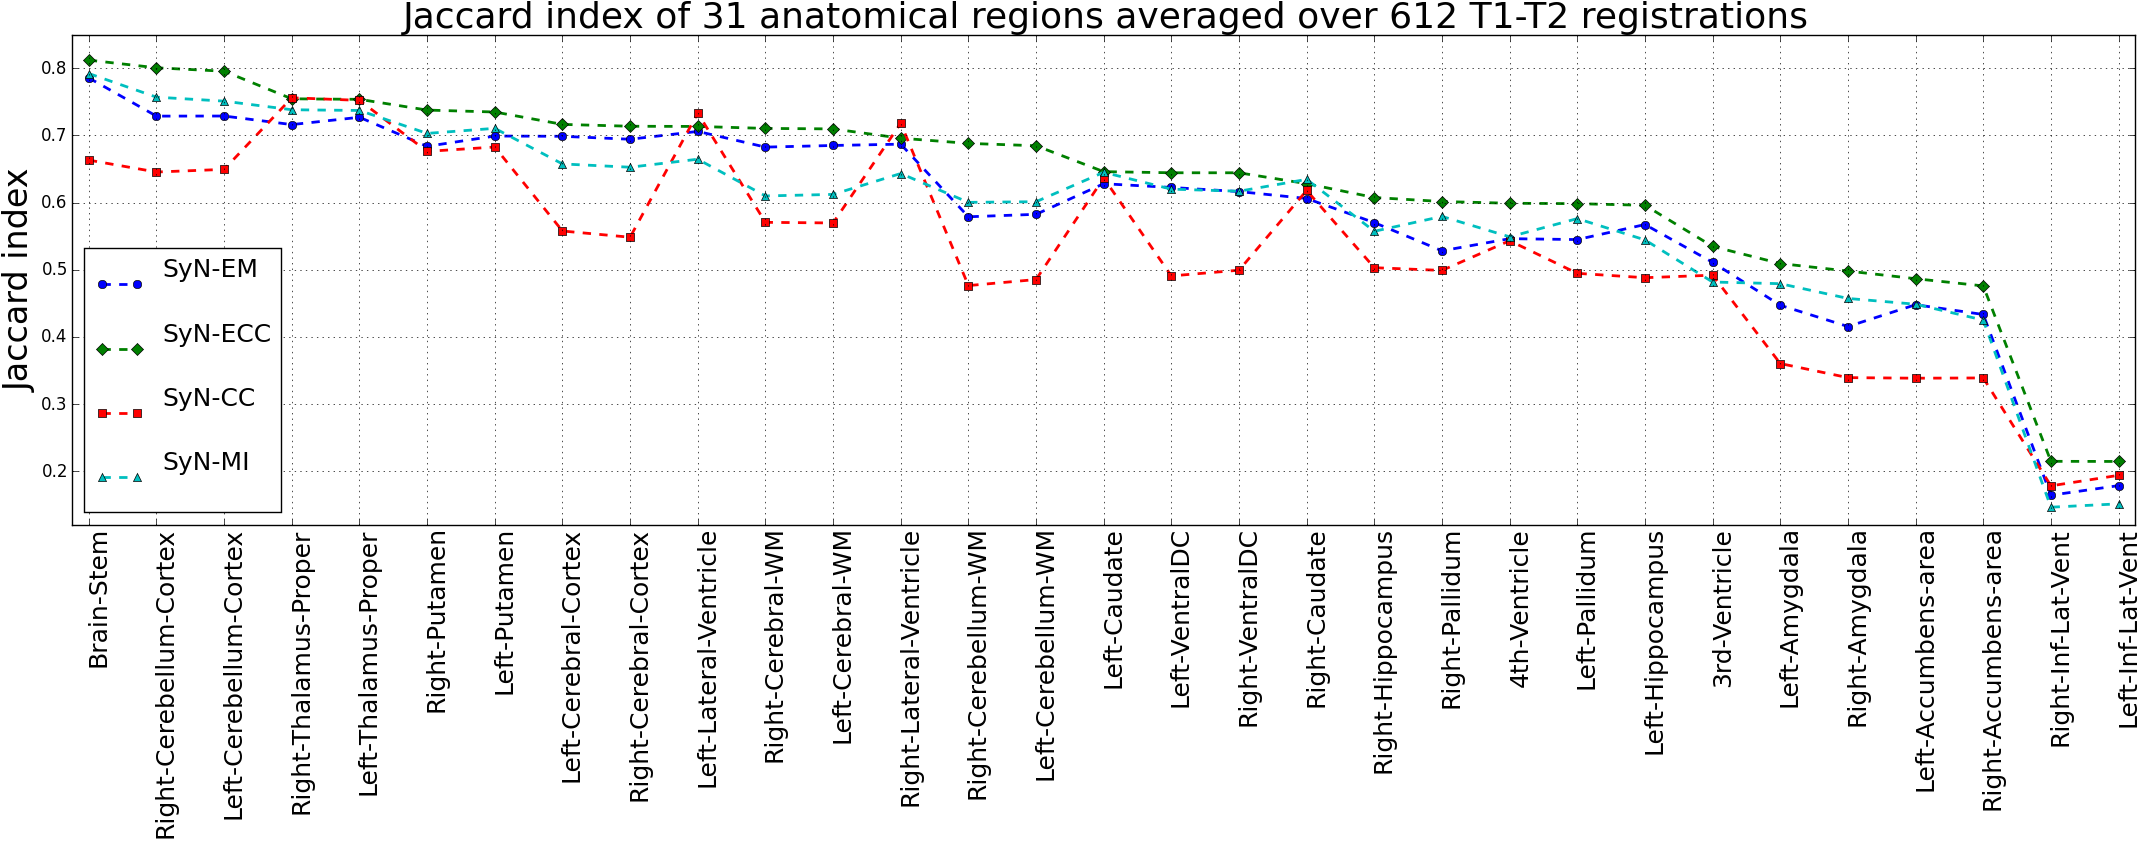
\includegraphics[width=1.0\linewidth]{./images/multi_lines_seg.png}\\
\caption{Comparison of the registration performance (measured by the Jaccard index over 31 anatomical regions) of the Greedy SyN algorithm with EM, ECC, CC and MI metrics. The Jaccard
indices were averaged over 612 multimodal registrations.}
\label{fig:multi_seg}
\end{figure}

\begin{figure}[H]
\centering
    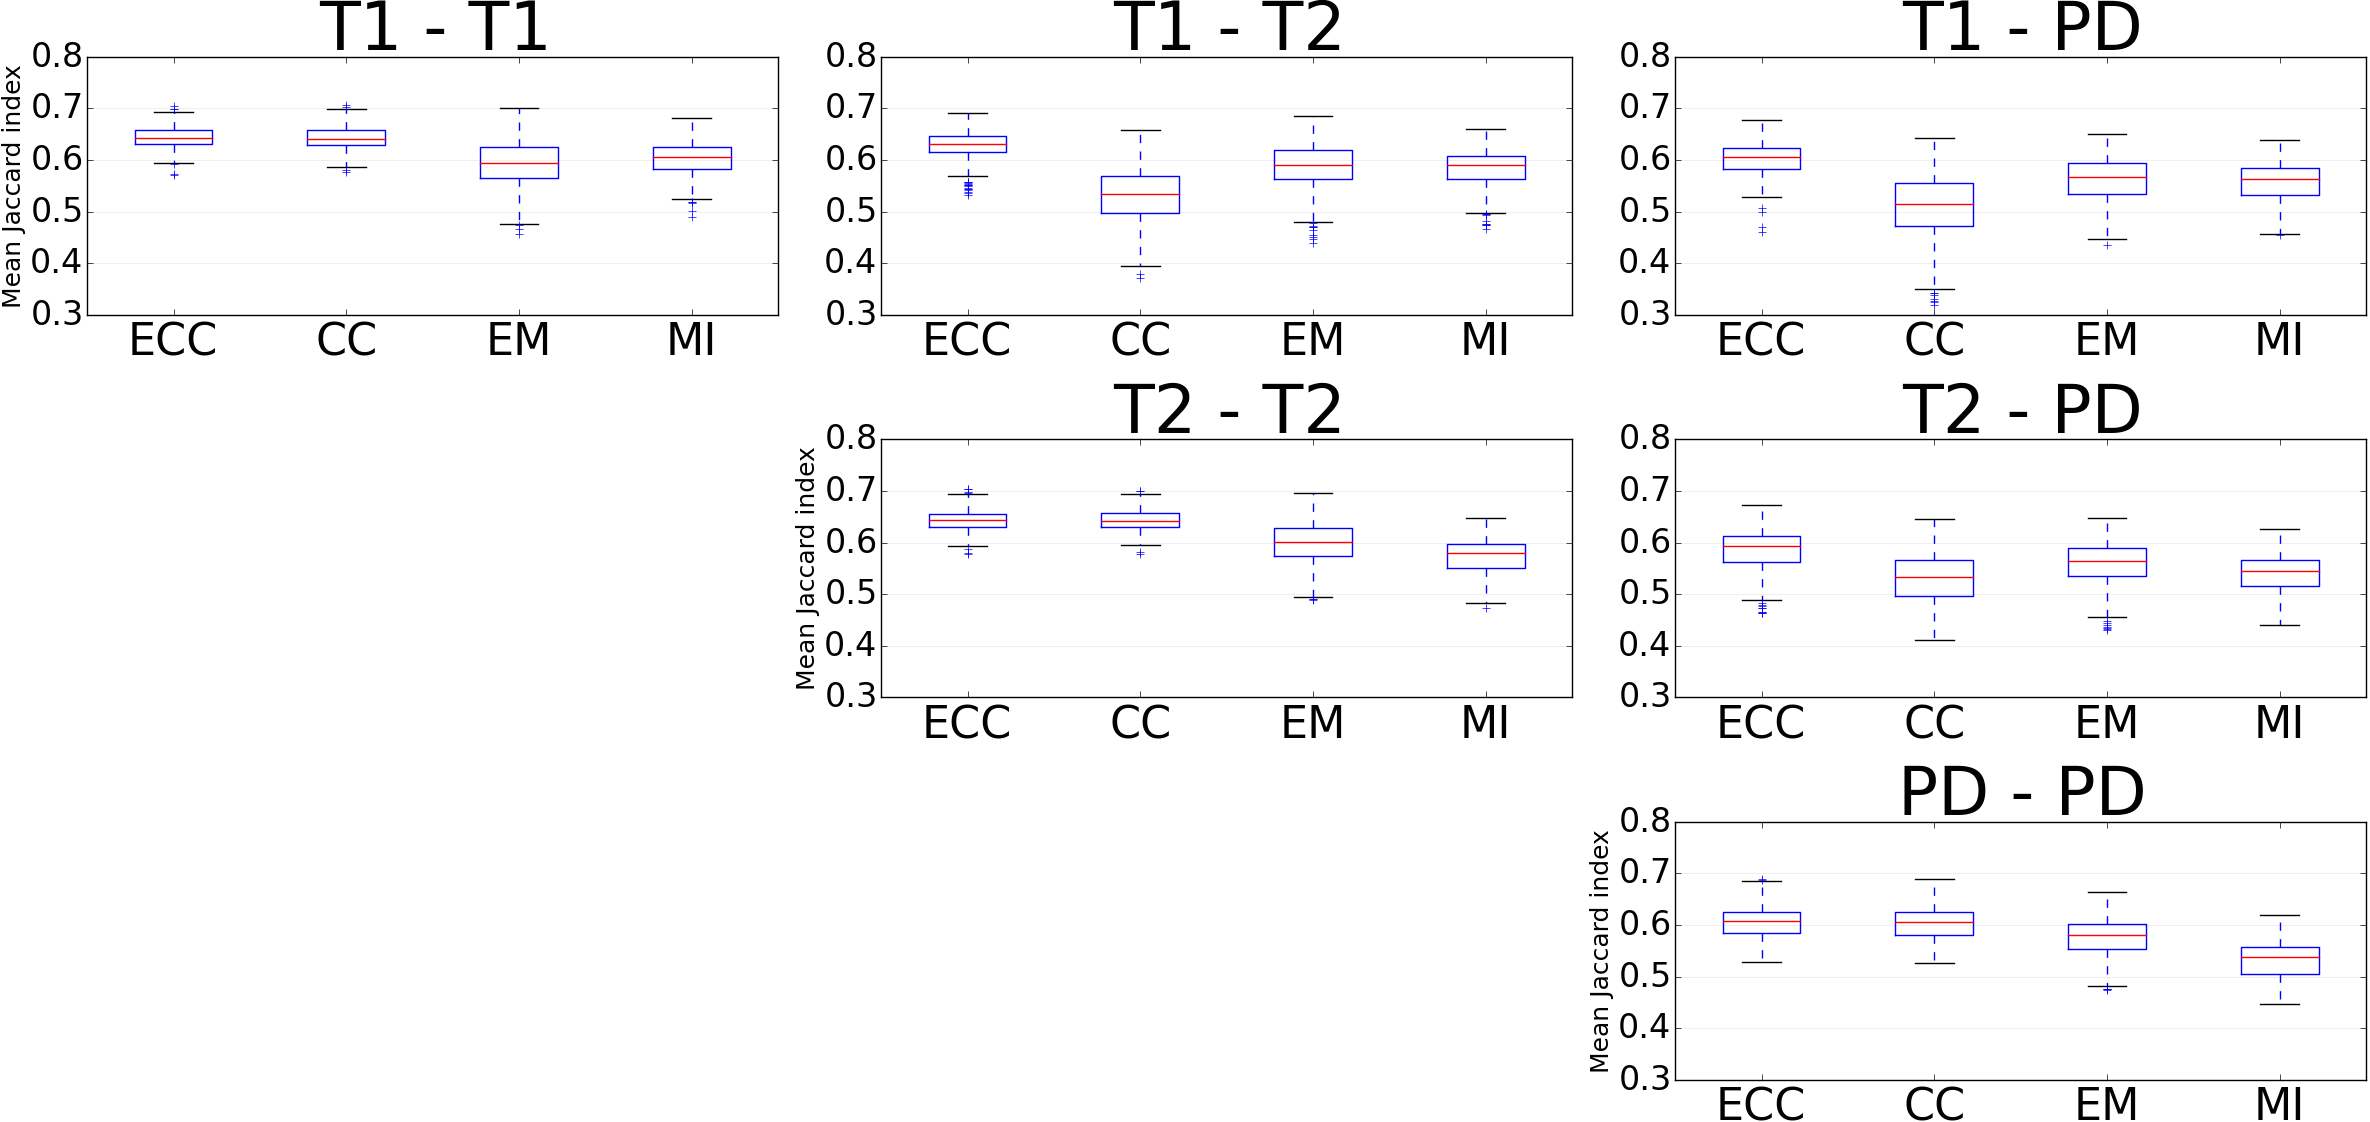
\includegraphics[width=\linewidth]{./images/all_modality_pairs_boxplots.png}
    \caption{Distributions of average Jaccard indices for all pairs of available modalities (T1, T2 and PD). For each pair of registrations, we compute the average Jaccard index of all anatomical regions. The boxplots show the distribution of all such average overlap scores.}
\label{fig:all_pairs_boxplots}
\end{figure}
